%% LyX 1.6.2 created this file.  For more info, see http://www.lyx.org/.

\documentclass[english]{IEEEtran}
\usepackage[T1]{fontenc}
\usepackage[latin9]{inputenc}
\usepackage{float}
\usepackage{textcomp}
\usepackage{amsthm}
\usepackage{amsmath}
\usepackage{graphicx}

\makeatletter

%%%%%%%%%%%%%%%%%%%%%%%%%%%%%% LyX specific LaTeX commands.
\newcommand{\noun}[1]{\textsc{#1}}
%% Because html converters don't know tabularnewline
\providecommand{\tabularnewline}{\\}
\floatstyle{ruled}
\newfloat{algorithm}{tbp}{loa}
\floatname{algorithm}{Algorithm}

%%%%%%%%%%%%%%%%%%%%%%%%%%%%%% Textclass specific LaTeX commands.
\theoremstyle{plain}
\newenvironment{lyxcode}
{\par\begin{list}{}{
\setlength{\rightmargin}{\leftmargin}
\setlength{\listparindent}{0pt}% needed for AMS classes
\raggedright
\setlength{\itemsep}{0pt}
\setlength{\parsep}{0pt}
\normalfont\ttfamily}%
 \item[]}
{\end{list}}

\@ifundefined{showcaptionsetup}{}{%
 \PassOptionsToPackage{caption=false}{subfig}}

\usepackage{subfig}
%\usepackage{subfloat}
\makeatother

\usepackage{babel}

\begin{document}

\title{Using Python in Computer Vision: Approach, Performance and Usability}

\author{Brian Thorne, Raphael Grasset, Richard Green\\
HIT Lab NZ, University of Canterbury, Private Bag 4800, Christchurch\\
Email: \{brian.thorne|raphael.grasset|richard.green\}@hitlabnz.org}
\maketitle

%matlab + pygpu
%importance of well written code, multi-thread optimization
%development and implementation time, documentation quality library, support
%declared and typed variable
%high level language, easy to read and understand (memory management, data storage format)
%PyPy py2exe, freeze
%GBLAS, GSL, Numerical Recipes in C
%http://old.scipy.org/documentation/weave/weaveperformance.html
%scientific/numerical computing

\begin{abstract}
Python is a popular language widely used by the scientific community due
to its clear syntax and an extensive number of specialized packages. For image 
processing or computer vision development, two libraries are prominently used:
\textit{NumPy/SciPy} and a python wrapper of \textit{OpenCV}. In this paper, we present a comparative 
evaluation of both libraries, assessing their performance as their usability. We also 
describe how Python implementation of OpenCV performs in comparison of the C++ implementation.
Our lessons learnt as a list of recommendations for the scholar community are also presented.
\end{abstract}

\begin{keywords}
Computer Vision, Python, OpenCV, SciPy
\end{keywords}

\section{Introduction}

Python \cite{} has been growing of interest by the academic community over the last decade.
The increase of computational science as a scientific method drives the need for scientists
to implement different mathematical models or simulation processes. The simple syntax of python, the absence
of data typed or management of hardware resources (e.g. memory management) has retained their attention
and forged it as a popular tool for the research community.

Differently, the field of image processing and computer vision (CV) has been driven for the last
decade by C/C++ implementation or the usage of MATLAB \cite{}. As MATLAB offers a really efficient 
high level platform for prototyping and testing algorithms, its performances doesn't compete with a well
designed and optimized C++ implementation. More recently, we have seen the emergence of potential
and valuable solution for developing image processing and computer vision algorithms in Python.

The goal of this paper is to evaluate the quality of the most common solution for developing 
CV algorithms and CV applications in Python. The outcomes of this evaluation aim to help on any decisional process
for shifting to future CV development in Python from the traditional approach. 

We were particularly interested to learn how Python performs in comparison of the native C implementation. We also focused our attention on the performances of two widely used CV libraries in Python: \textit{OpenCV}\cite{} and \textit{NumPy/SciPy}\cite{oliphant2007python}. For this matter, we analyzed their performances through a list of common tasks and processes regularly employed in 
computer vision (e.g. video capture, filtering algorithms, feature detection, etc). 

After an introduction of our experimental process, we will describe the list of tested CV tasks and algorithms
and finally discuss our findings and provide recommendations.

\section{Experimental Process}

In this section, we briefly introduce the different libraries we tested as our 
experimental protocol.

\subsection{Background}

\textbf{Python}

\textit{Python} is a general purpose dynamic programming language\cite{entry-0}.
It is highly regarded due in no small part for its fast development
time and easiness for integrating third-parties packages\cite{sanner1999python}.
Python's performance makes it a viable programming language for scientific
work \cite{cai2005performance}. It has been used by a few people in
Computer Vision for many years \cite{doakPyCV}.



\textbf{OpenCV}

Originally an Intel research initiative, \textit{OpenCV} cross-platform open
source computer vision library is widely used for real time image processing.
It aims to provide well tested, optimized and open source code for image
processing and computer vision. 

The library is written in C, ensuring both fast and portable code (optionally
to embedded platforms). The library is using a base layer related to image structure
and basic image manipulation. A software implementation is provided freely whilst an accelerated
version (\textit{IPP, Integrated Performance Primitives}\cite{}) can be optionally acquired 
from Intel. This latter takes benefit of extended multimedia instruction set available on 
Intel Processors.

Nowadays, multiple language bindings are available for OpenCV, as XX, XX and multiple
for Python (\cite{}, \cite{}).



\textbf{NumPy/SciPy}

\textit{NumPy} package delivers N-dimensional arrays support for Python\cite{oliphant2006guide}.It's a well
recognized library offering very fast raw data crunching, iterating, and an easier approach
for multidimensional matrices manipulation than in C language.

\textit{SciPy} \cite{jones2001scipy} is a set of Python libraries and tools
for scientific and mathematical work built on top of NumPy \cite{oliphant2007python}.
SciPy offers different filters algorithms, XX, XX. This leads to much elegant code, usually recognized as not impacting
significantly a performance loss over C. Two major tools usually distributed with
SciPy are very useful for computer vision development:  matplotlib and ipython. 
Matplotlib\cite{hunter2007matplotlib} is a matrix plotting library, and Ipython is an improved interactive shell for Python\cite{perez2007ipython}.

\subsection{Evaluation}

We conducted our test on a XXX MACHINE, XXX RAM, with XXX OS XXX version. For the test we compared:
\begin{itemize}
	\item OpenCV Native Language (ACRONYM): we used snapshot built version 1.1.1, rev 1978. The code
	has been compiled with XXX and in mode XXX.
	\item OpenCV Python Wrapper (ACRONYM): we used the swig\cite{beazley1996swig} wrapper. We used 
	similar version as the native language.
	\item SciPy/NumPy (ACRONYM):we used XXX.
\end{itemize}

The list of tests we are not only covering different standard algorithms traditionally used in a
CV application but also some standard operations used in CV as video grabbing or image recording. For each
of the test we describe the process, the difference in term of syntax as the performance and usability.

Notice that for some tests we were only able to compare 2 of the 3 libraries (REWRITE THAT).

\section{Tests}

\subsection{Image Acquisition}

The first thing to think about in computer vision programs is where
the image data comes from. In this report mostly just live data from
a web-cam is under consideration. The main difference in using a live
system is the time available for processing is very constrained to
allow a frame rate sufficient for live viewing. Processing on static
images or recorded video data doesn't have this constraint.

\subsubsection{Acquiring and displaying an image in C with OpenCV}

Algorithm \ref{alg:C-Image-capture} opens up a new camera capture
device, and takes one frame, it creates a new window and displays
it%
\footnote{For brevity these code snippets do not carry out error checking or
cleanup. It is assumed that a camera was found successfully and that
a frame was available and returned. The C++ and Python versions of
VideoCapturePlayer do carry out this error checking.%
}. Using this as a template it is straight forward to wrap the capture
and display in a loop, this forms the basis of the C++ class \noun{VideoCapturePlayer}
included in the appendix. This \noun{VideoCapturePlayer} class is
used in the other examples to keep the code duplication and variation
to a minimum.

%
\begin{algorithm}[h]
\begin{lyxcode}
\#include~\textquotedbl{}cv.h\textquotedbl{}

\#include~\textquotedbl{}highgui.h\textquotedbl{}

int~main()\{

~~IplImage~~{*}frame;

~~CvCapture~{*}capture;

~~capture~=~cvCreateCameraCapture(0);

~~cvNamedWindow(~\textquotedbl{}Snapshot\textquotedbl{},~0~);

~~frame~=~cvQueryFrame(~capture~);

~~cvShowImage(~\textquotedbl{}Snapshot\textquotedbl{},~frame~);

\}
\end{lyxcode}
\caption{\label{alg:C-Image-capture}Image capture and display with OpenCV
in C. }

\end{algorithm}

%
\begin{algorithm}[h]
\begin{lyxcode}
from~opencv~import~highgui~as~hg

capture~=~hg.cvCreateCameraCapture(0)

hg.cvNamedWindow(\textquotedbl{}Snapshot\textquotedbl{})

frame~=~hg.cvQueryFrame(capture)

hg.cvShowImage(\textquotedbl{}Snapshot\textquotedbl{},~frame)
\end{lyxcode}
\caption{\label{alg:Python-Image-capture}Image capture and display in Python}

\end{algorithm}


\subsubsection{Acquiring and displaying an image in Python with OpenCV}

Algorithm \ref{alg:Python-Image-capture} does the same basic task
of accessing a webcam and displaying one image in Python. The code
is almost entirely identical in C and Python. The main difference
being in the Python code no variables types are declared, this shows
the dynamic nature of the language. As with C++, an object orientated
version of this acquisition loop with error checking is used in further
tests. The \noun{VideoCapturePlayer} classes in both C++ and Python
optionally take a function as an argument. This function takes the
raw image, does some process on it, and returns an image for display. 


\subsubsection{Comparison}

Table \ref{tab:IO-bound-Webcam} shows results for taking an image
from a webcam and displaying the image with OpenCV. The average frames
per second are taken over 3 trials each averaging over a 2 minute period.

%
\begin{table}
\caption{\label{tab:IO-bound-Webcam}Simple IO bound test - Webcam streaming
comparison of Python and C++. Results shown are in frames per second.}


\begin{centering}
\begin{tabular}{|c|c|c|c|c|c|}
\hline 
Language & Run 1 & Run 2 & Run 3 & Mean & Std Dev\tabularnewline
\hline
\hline 
Python & 15.007 & 15.003 & 15.007 & 15.006  & 2.25E-03 \tabularnewline
\hline 
C++ & 15.017 & 15.009 & 15.010 & 15.012  & 4.27E-03 \tabularnewline
\hline
\end{tabular}
\par\end{centering}


\end{table}


As the results in Table \ref{tab:IO-bound-Webcam}and Figure \ref{fig:Streaming-comparison}
show, Python and C++ perform at very similar rates whilst carrying
out an I/O bound task. The not unexpected result points at C++ having
a marginally higher frame rate output than Python. 

%
\begin{figure}[h]
\centering{}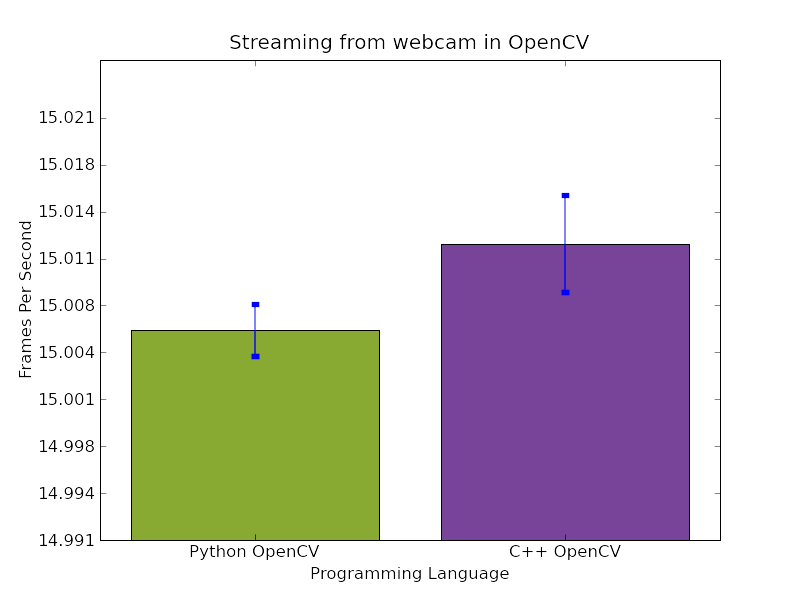
\includegraphics[width=0.8\columnwidth]{report_data/streaming_from_webcam_in_opencv}\caption{\label{fig:Streaming-comparison}Comparison of Python and C++ performance
using OpenCV for webcam capture and display.}

\end{figure}



\subsection{Image Blur}

One of the simplest operations in image processing is blurring an
image. This can be achieved in a few ways, the method looked at here
is by adding gaussian blur. Mathematically this is achieved by convolving
the image with a gaussian filter. Because of the separability of multidimensional
gaussian filters\cite{young1995recursive}, the convolution can be
applied in two ways; applying a 1 dimensional filter twice, once in
each direction; or secondly the image can be convolved with a 2-dimensional
gaussian filter created by the product of two 1 dimensional filters.
Equation \ref{eq:1D Gaussian Filter} shows the gaussian function
for obtaining the filter is in one dimension\cite{SS01}. \begin{equation}
G\left(x\right)=\frac{1}{\sqrt{2\pi}\sigma}e^{-\frac{x^{2}}{2\sigma^{2}}}\label{eq:1D Gaussian Filter}\end{equation}
\begin{equation}
G\left(x,y\right)=\frac{1}{\sqrt{2\pi}\sigma^{2}}e^{-\frac{x^{2}+y^{2}}{2\sigma^{2}}}\label{eq:2D Gaussian Filter}\end{equation}
Equation \ref{eq:2D Gaussian Filter} shows the 2 dimensional case\cite{SS01}.
OpenCV includes a gaussian filter that can be applied to an image
by calling the \emph{\noun{cvSmooth}} function and passing the desired
window size. SciPy has a n-dimensional Gaussian filter that acts on
a NumPy array. Both libraries use the 1 dimensional case, as it requires
less calculations.


\subsubsection{C++}

Algorithm \ref{alg:Gaussian-C} shows calling the OpenCV function
\noun{cvSmooth} to carry out gaussian blur with a filter size of 43. 


\subsubsection{Python}

Algorithm \ref{alg:Gaussian-Python-OpenCV} shows Python taking advantage
of VideoCapturePlayer, the Python class introduced earlier in this
document, to do the same blurring operation with OpenCV%
\footnote{A helper function here calculates the sigma value to use in the convolution,
this is usually done automatically in OpenCV, but to port to SciPy
the parameters must all be known.%
}. Algorithm \ref{alg:Gaussian-Python-SciPy} is also using the VideoCapturePlayer
but this time using SciPy instead of OpenCV to do the convolution.
To continue using the OpenCV camera capture, the image data must be
converted into NumPy arrays; this has been achieved here by creating
and using a Python decorator which converts before and after calling
a Python function using NumPy. A (640x480) RGB image takes less than
2ms to convert either way on the testing platform used throughout
this report. Also the filter parameters need converted to be compatible
with OpenCV's \noun{cvSmooth} defaults\cite{bradski2008learning}.


\subsubsection{Comparison}

As expected the images produced by this are blurred as shown in figure
\ref{fig:Gaussian-Output-Images}. For qualitative comparison a static
input image was used. What is not immediately obvious without further
investigation is how similar the results are. The OpenCV images produced
by C++ and Python are exactly the same pixel for pixel, this is expected
because the same function is doing the filtering. More interesting
is figure \ref{fig:Difference-in-Python} which shows that the SciPy
and OpenCV Python code doing the filtering produces very similar but
slightly different results. This could be caused by the discretization
at the precission limit of the image, or the floating point nature
of the convolution as the difference is very small. It may be due
to a type difference or another possible small effect would be caused
by a difference in the algorithms. Possibly since SciPy uses the sigma
parameter, the filter is created by direct sampling of the Gaussian
function. OpenCV on the other hand, uses the size of the filter, this
is a good indication it probably uses the pascal triangle which is
another good approximation for the Gaussian kernel\cite{ben1991image}.
Whatever the reasons, the differences are negligible.

The graph itself in figure \ref{fig:Difference-in-Python} is worth
a mention, because it shows a 3 way sub plot of a single image made
inplace with the Python plotting package matplotlib directly on the
data from OpenCV. This means that as a researcher to debug a misbehaving
programmer you can just jump right into the middle of a deeply nested
loop, introspect all variables, plot any signal or image, call any
function, accuratly time any function.

%
\begin{algorithm}[H]
\begin{lyxcode}
from~IPython.Shell~import~IPShellEmbed~

IPShellEmbed()()
\end{lyxcode}
\caption{\label{alg:drop-to-shell}Two lines of Python code can be put anywhere
in a computer vision program and it will pause execution and drop
into a live interactive shell with full plotting capabilities.}



\end{algorithm}


%
\begin{figure}[h]
\begin{centering}
\subfloat[C++]{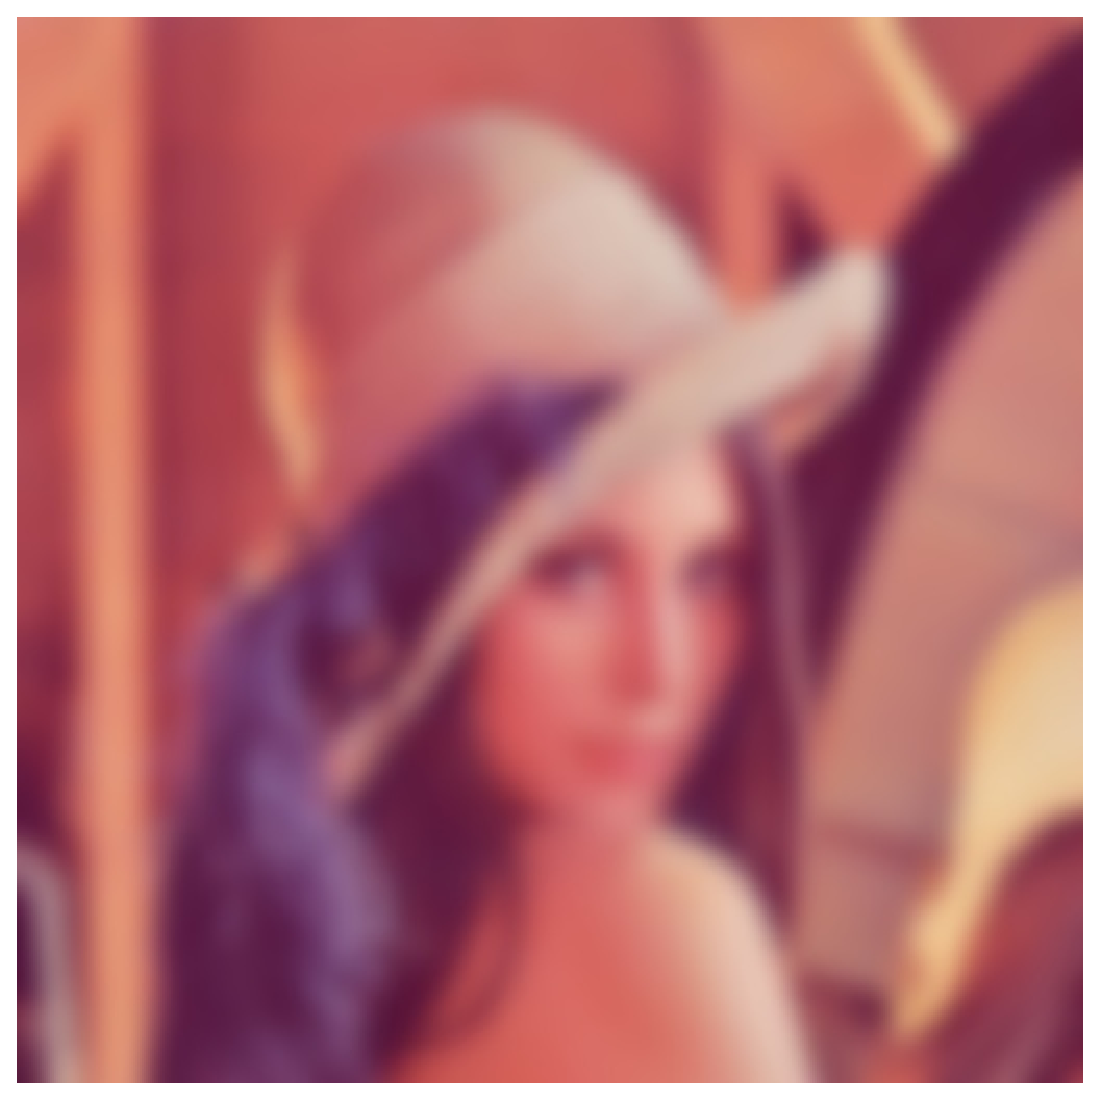
\includegraphics[width=0.3\columnwidth]{report_data/blurred_imag_cpp_opencv_gaussian}



}\subfloat[Python OpenCV]{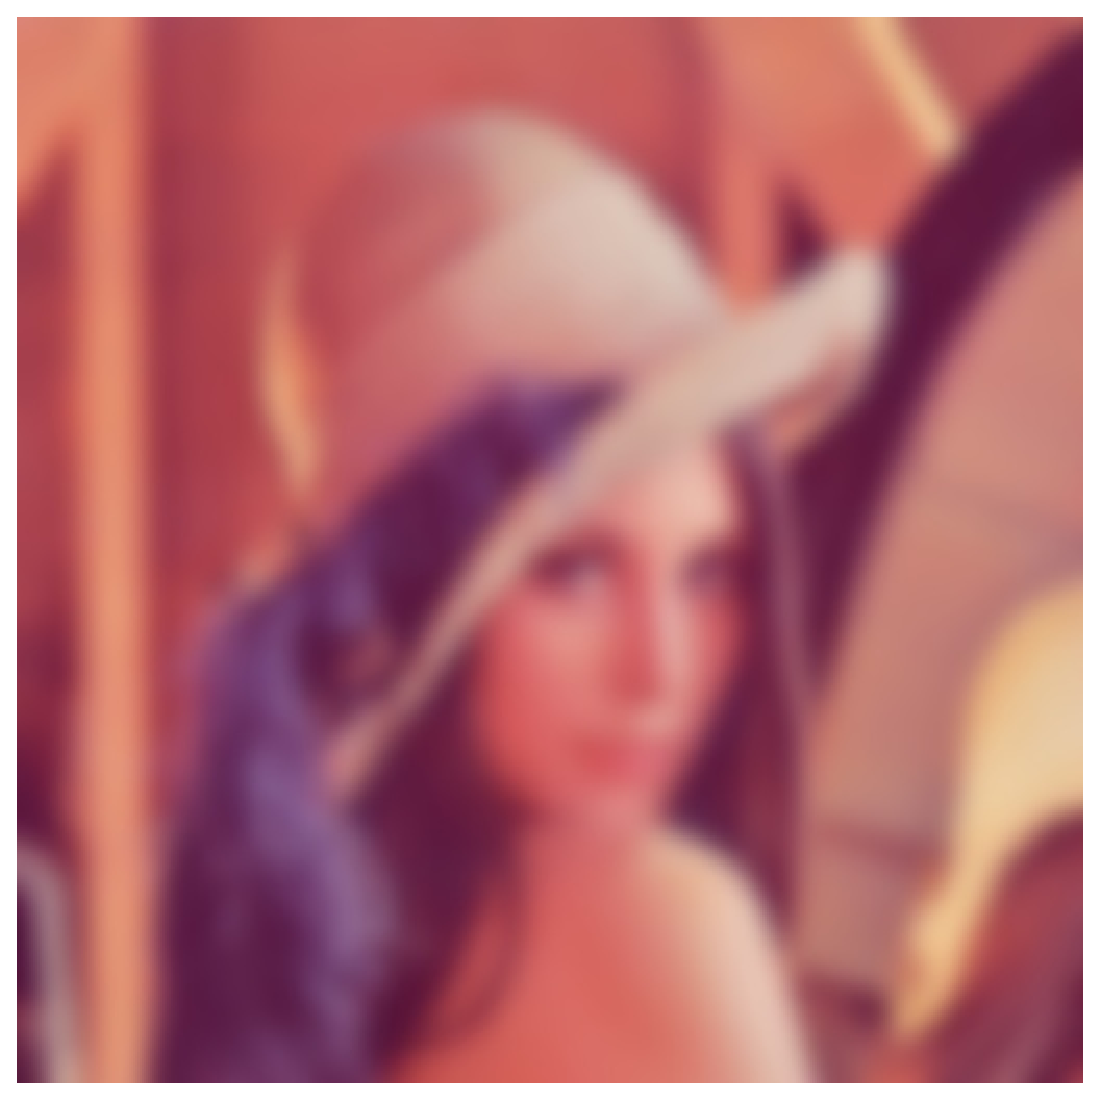
\includegraphics[width=0.3\columnwidth]{report_data/blurred_imag_python_opencv_gaussian}



}\subfloat[Python SciPy]{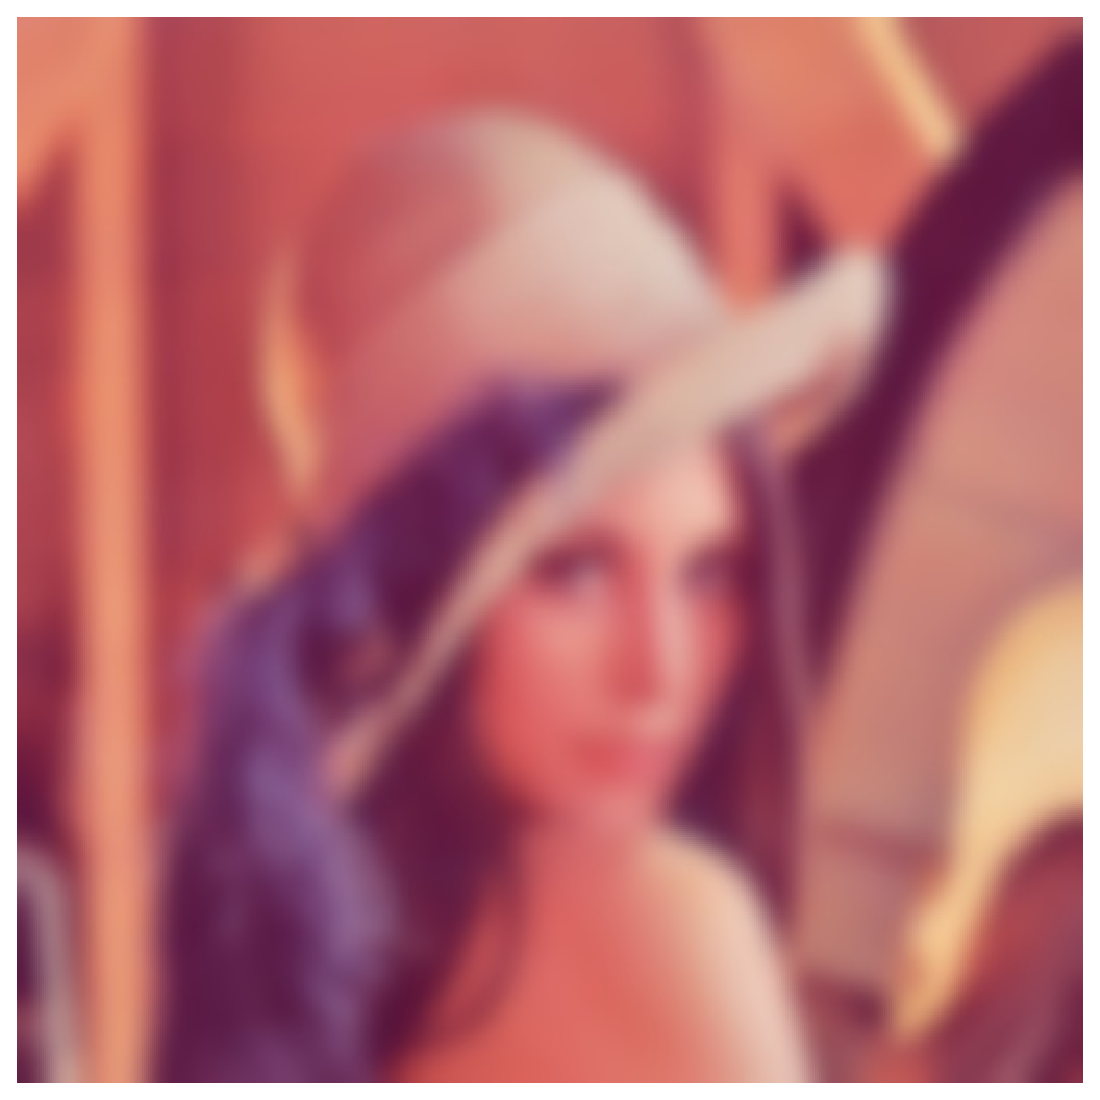
\includegraphics[width=0.3\columnwidth]{report_data/blurred_imag_python_scipy_gaussian}



}
\par\end{centering}

\subfloat[\label{fig:Difference-in-Python}Difference of each channel after
gaussian blur in OpenCV and SciPy. Note full scale is 255, Pixel for
pixel difference image stats: maximum intensity difference = 20, average
difference = 2.1. with std dev = 1.4]{\begin{centering}
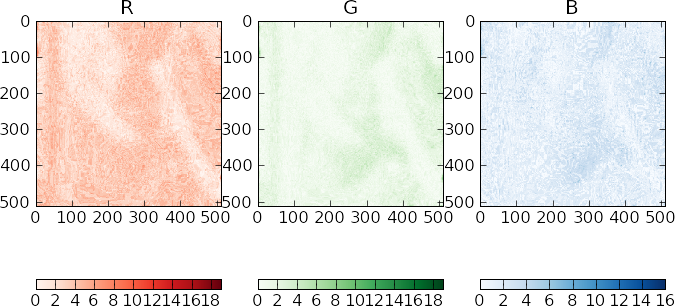
\includegraphics[width=0.95\columnwidth]{report_data/gaussian_diffs}
\par\end{centering}

}

\caption{\label{fig:Gaussian-Output-Images}Output Images from Gaussian Blur
Examples}

\end{figure}
%
\begin{table}
\caption{\label{tab:Gaussian-Results}CPU bound test results - Gaussian Blur
filtering on webcam stream (in fps)}


\centering{}\begin{tabular}{|c|c|c|c|c|c|}
\hline 
Language & Run 1 & Run 2 & Run 3 & Mean & Std Dev\tabularnewline
\hline
\hline 
Python & 14.555 & 14.737 & 13.989 & 14.427 & 0.318\tabularnewline
\hline 
C++ & 14.722 & 14.627 & 14.612 & 14.653 & 0.049\tabularnewline
\hline 
SciPy & 4.374 & 4.3886 & 4.337 & 4.3664 & 0.0219\tabularnewline
\hline
\end{tabular}
\end{table}
%
\begin{figure}[H]
\begin{centering}
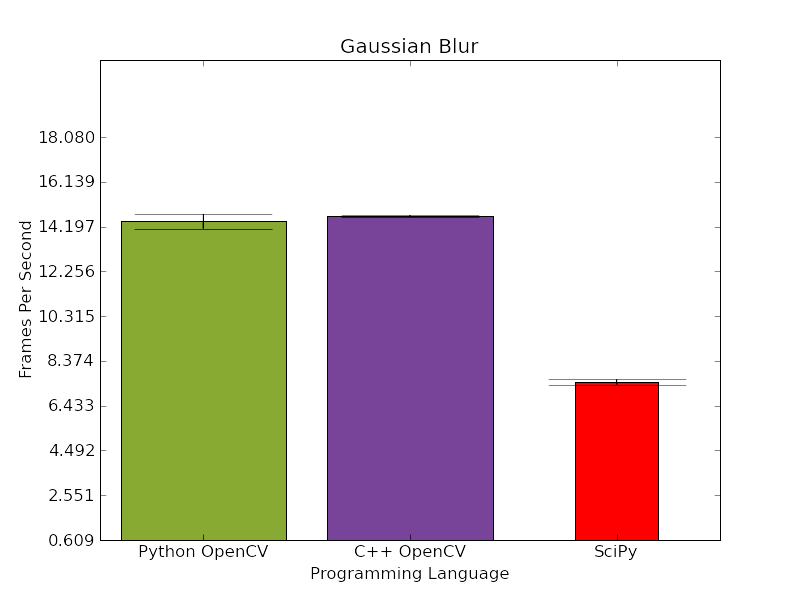
\includegraphics[width=0.8\columnwidth]{report_data/gaussian_blur}
\par\end{centering}

\caption{\label{fig:performance-gaussian}OpenCV performance carrying out Gaussian
Blur}



\end{figure}



\subsection{Background subtraction}

To detect movement in a video, a comparison of a frame to a previous
frame must be undertaken\cite{gao2006robust}. This can be done quite
straighforwardly by simply taking the absolute intensity difference
between those frames, pixel for pixel, across all channels. This gives
a difference image, which contains specific colour information about
the change of state. We need to filter this information, to only look
at points which have changed more than a set minimum. We do this by
applying a threshold, then removing salt and pepper noise with a median
filter, the output from this is a multichannel binary image. Then
create a new black image, to render the movement data on. Then for
every point in the binary difference image, if any of the channels
are true, copy the original point data from the current frame onto
the black image. And thus we have a colour image of only what has
changed. The response is shown in figure \ref{fig:Adding-a-single}
after adding a cellphone to the scene for the Python implementation
in algorithm \ref{alg:back-Python-imple}. 

%
\begin{figure}[h]
\subfloat[\label{fig:Adding-a-single}Adding item]{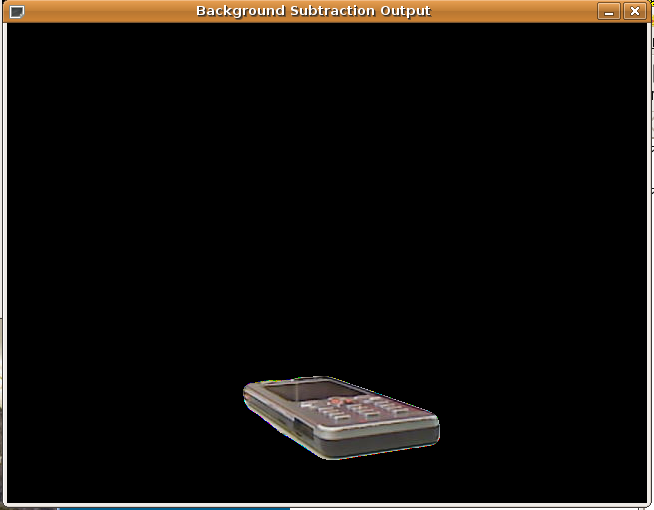
\includegraphics[width=0.3\columnwidth]{report_data/background_python_add_item}}\subfloat[\label{fig:Adding-another-item,}minor problems]{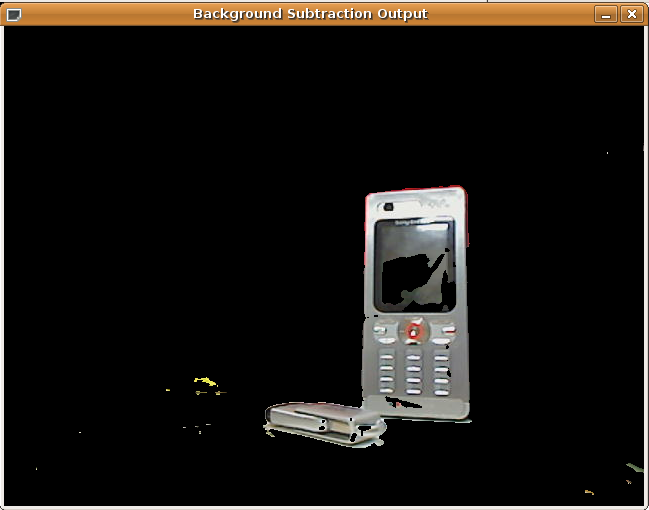
\includegraphics[width=0.3\columnwidth]{report_data/background_python_add_more_items}

}\subfloat[\label{fig:remove-laptop}Addition and removal]{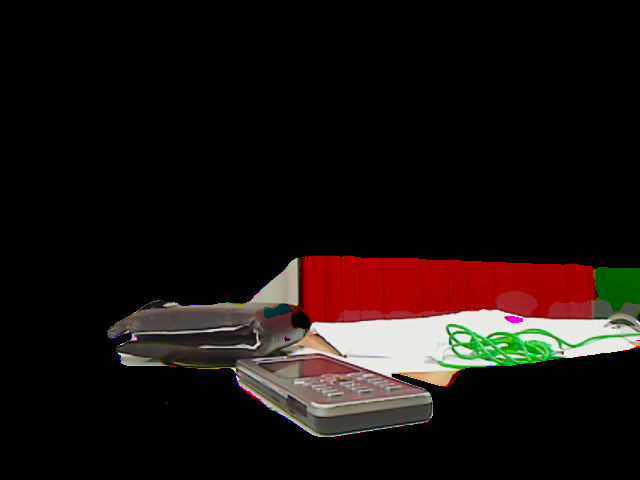
\includegraphics[width=0.3\columnwidth]{report_data/background_python_add_remove_item}

}

\caption{\label{fig:background-Adding-and-removing}Background subtraction
response to adding and removing items from a scene.}

\end{figure}
%
\begin{figure}
\subfloat[before]{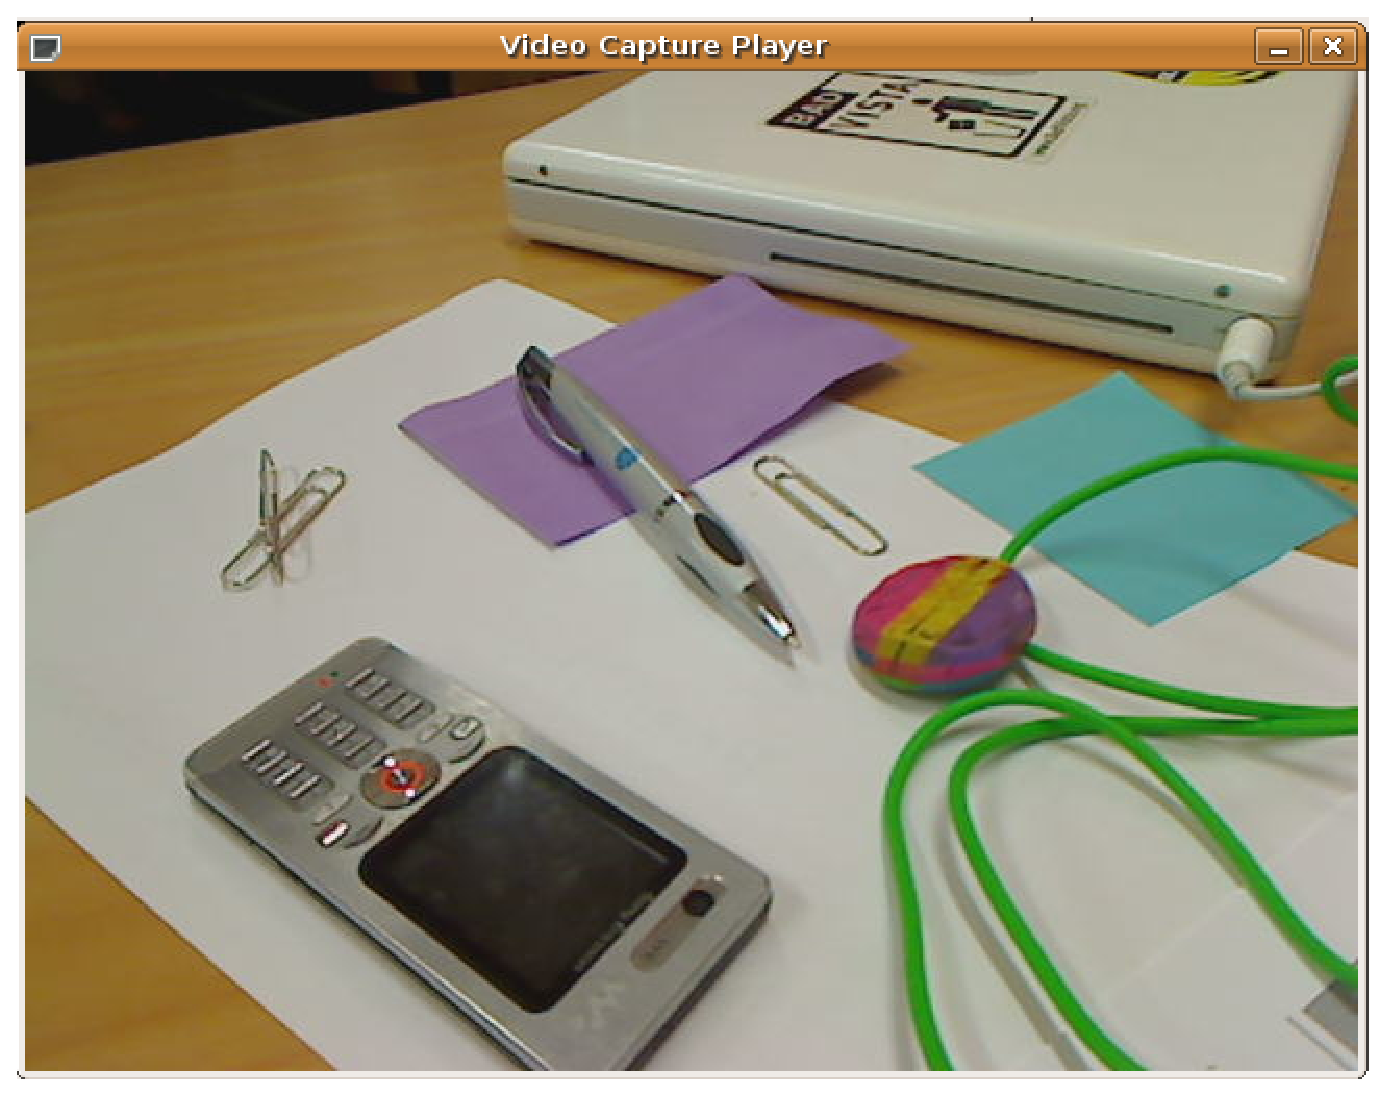
\includegraphics[width=0.3\columnwidth]{report_data/background_python_before}

}\subfloat[program output]{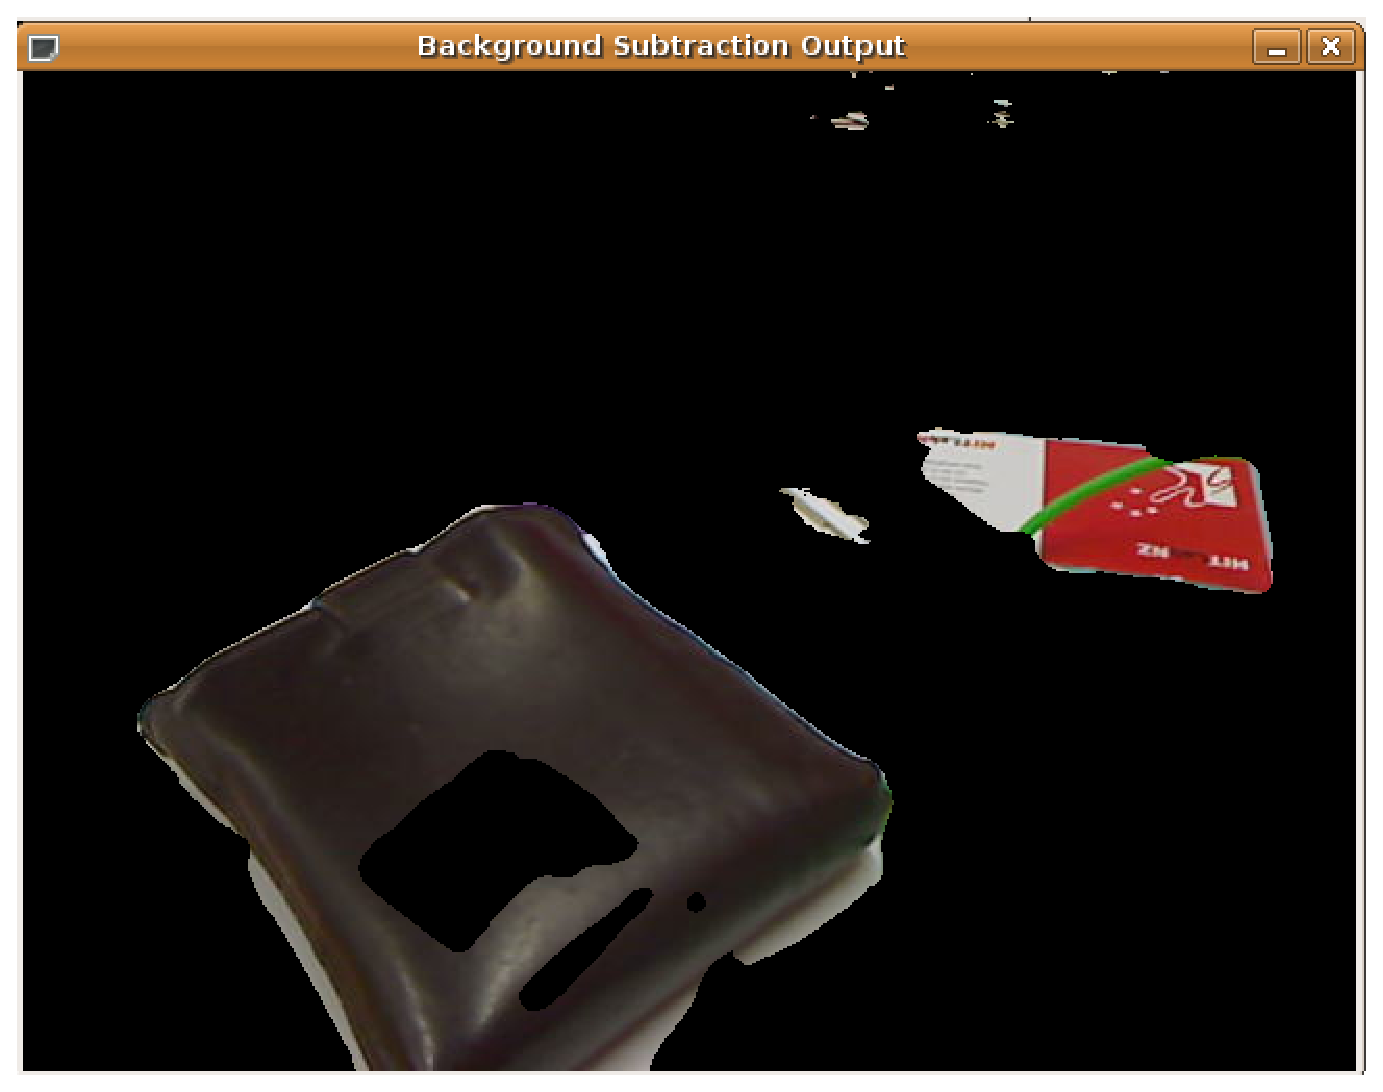
\includegraphics[width=0.3\columnwidth]{report_data/background_python_add_items_complicated}

}\subfloat[after]{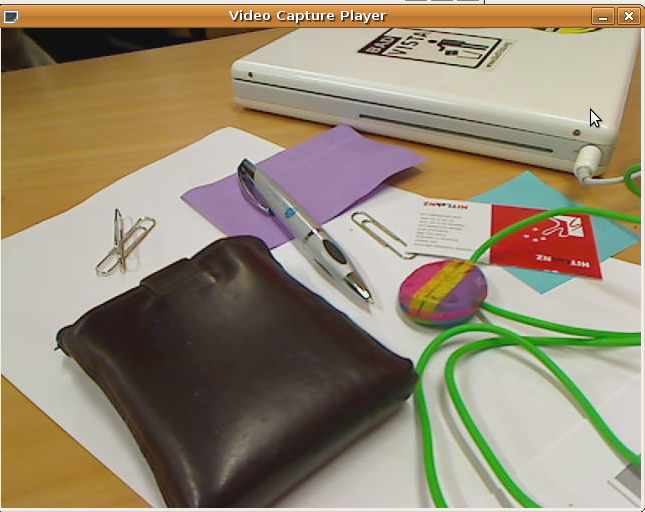
\includegraphics[width=0.3\columnwidth]{report_data/background_python_after}

}

\caption{\label{fig:back-Proces-clutter}Background subtraction response on
a cluttered scene where a cellphone is switched for a wallet and a
contact card is added.}

\end{figure}


Regions of the same colour, like pieces of paper make it more difficult
for this algorithm to work, the noise around the USB device in figure
\ref{fig:Adding-another-item,} is caused by moving the paper underneath
it. Only the edges are detected as having changed. Another issue is
shown in figure \ref{fig:remove-laptop}, although from visual inspection
one can see that something has changed to the right of the added wallet
and cellphone, it is almost impossible to identify that a laptop was
removed. This method could be improved by having a second view looking
at the changes applied in the same way to the original image. The
figures in \ref{fig:back-Proces-clutter} show how the algorithm deals
with a combination of changes. 

While creating this program I found algorithm \ref{alg:drop-to-shell}
particuly helpfull, it allows for interactive, inplace trialing, timing
and plotting as shown in algorithm \ref{alg:Interactive,-inplace-timing}.

%
\begin{algorithm*}
\begin{lyxcode}
\noindent In~{[}1{]}:~from~opencv~import~cv

\noindent In~{[}2{]}:~cv.cvAnd(differenceImage,image,~temp)

\noindent In~{[}3{]}:~timeit~cv.cvAnd(differenceImage,image,~temp)

\noindent 1000~loops,~best~of~3:~229~\textmu{}s~per~loop

\noindent In~{[}4{]}:~from~pylab~import~imshow,~show

\noindent In~{[}5{]}:~imshow(temp)~

\noindent Out{[}5{]}:~<matplotlib.image.AxesImage~object~at~0x42489d0>

\noindent In~{[}6{]}:~show()
\end{lyxcode}
\caption{\label{alg:Interactive,-inplace-timing}Using algorithm \ref{alg:drop-to-shell}
the interactive shell can be used from deep inside a nested loop.
Inplace timing and plotting with access to local variables and functions
like this example speeds up development time.}

\end{algorithm*}



\subsection{Feature Point Detection}

Many methods in computer vision for identifying the contents of an
image relies on extracting \emph{interesting} features. An interesting
feature point could be corners of intersecting lines, a line ending,
or any isolated point where local image regions have a high degree
of variation in all directions\cite{harris1988combined}. The features
must be found algorithmically and have a well-defined position. The
repeatability of choosing the same points under differing conditions
is a measure of how good an interesting feature algorithm is. The
corner detection algorithm works by locating points where the surroundings
have edges in more than one direction. According to \cite{Sol09}
the Harris \& Stephens algorithm is in short: 
\begin{quote}
A matrix W is created from the outer product of the image gradient,
this matrix is averaged over a region and then a corner response function
is defined as the ratio of the determinant to the trace of W.
\end{quote}
A threshold is then applied to this corner response image to pick
the most likely candidates and then these points are plotted. An example
usage of the algorithm is in the Lucas\textendash{}Kanade Optical
Flow Method where it can be used to select good feature points\cite{beauchemin1995computation}
for tracking movement.

%
\begin{figure}[h]
\begin{centering}
\subfloat[static image processing]{\begin{centering}
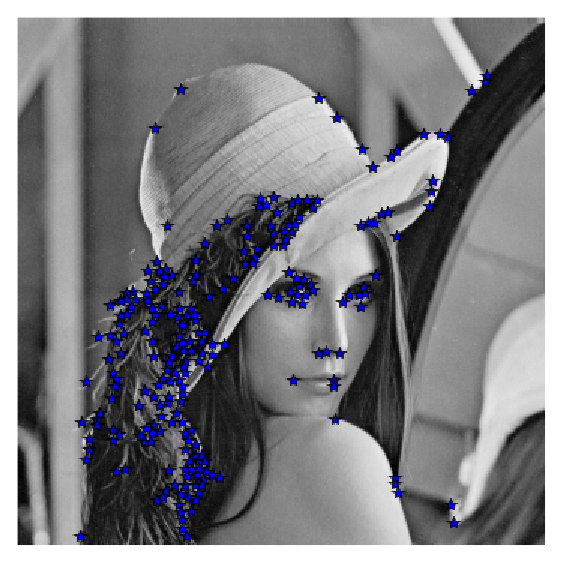
\includegraphics[width=0.45\columnwidth]{static_harris_file}
\par\end{centering}

}\subfloat[processing from webcam]{\begin{centering}
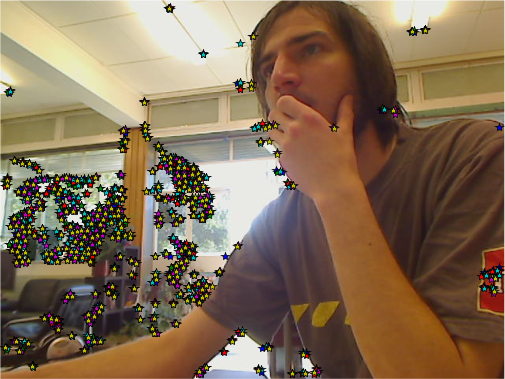
\includegraphics[width=0.45\columnwidth]{temp_harris_file_248_points}
\par\end{centering}

}
\par\end{centering}

\caption{\label{fig:A-SciPy-harris}A SciPy implementation of the Harris \&
Stephens feature detection algorithm.}

\end{figure}
%
\begin{figure}[h]
\begin{centering}
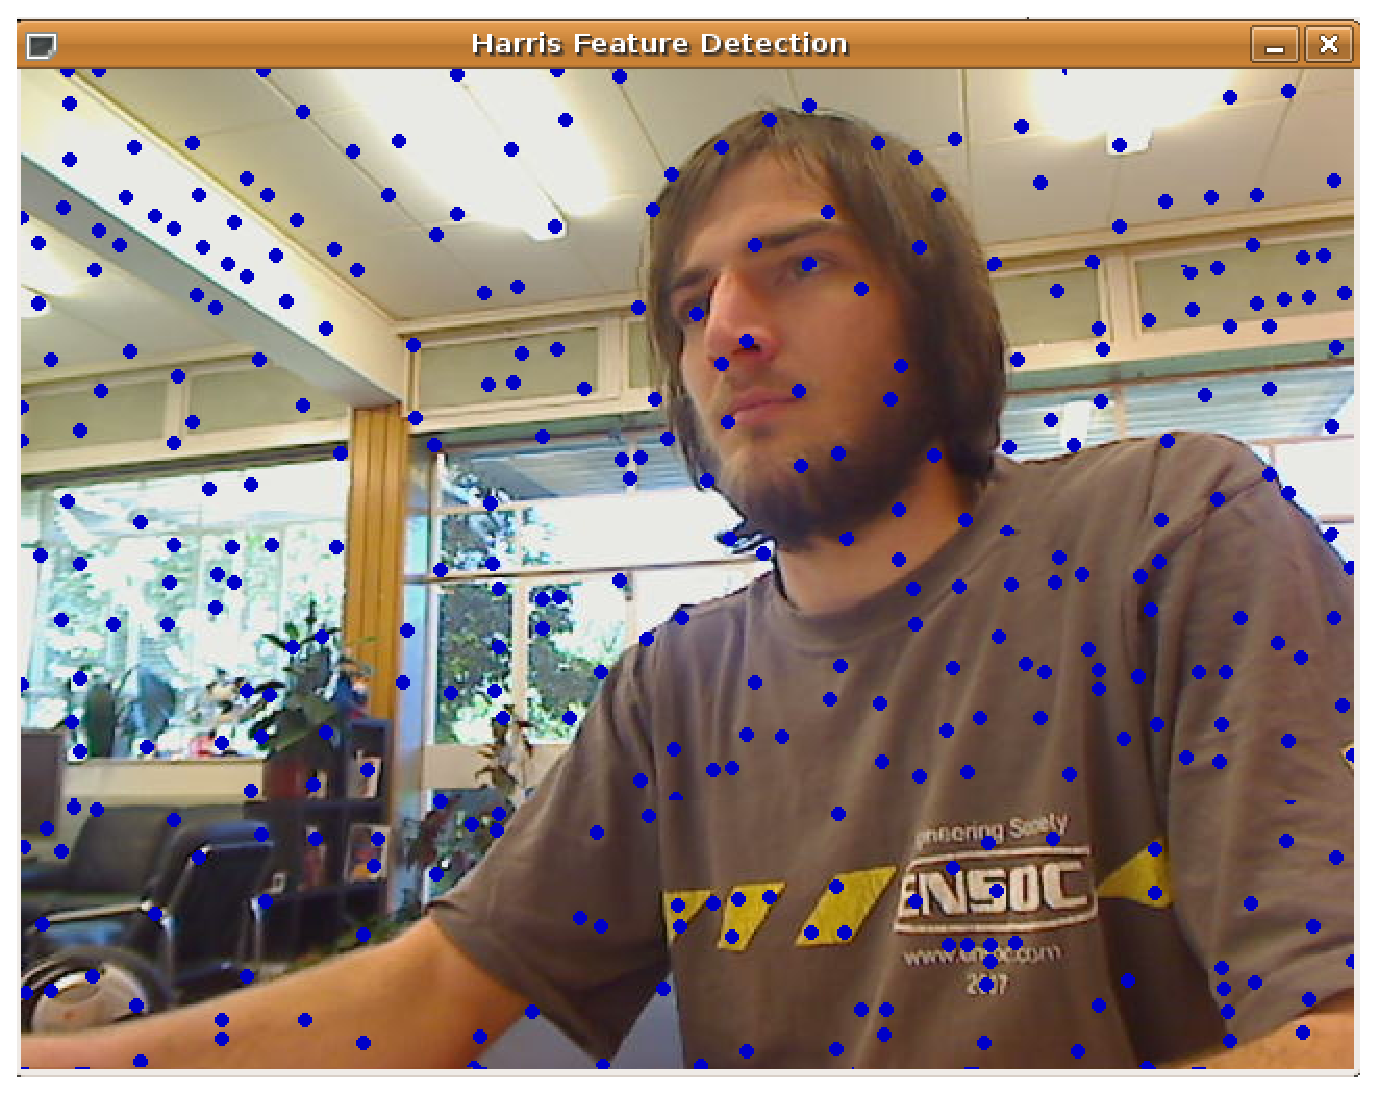
\includegraphics[width=0.9\columnwidth]{report_data/opencv_python_harris}
\par\end{centering}

\caption{\label{fig:OpenCV-harris}OpenCV implementation of the Harris \& Stephens
feature detection algorithm}

\end{figure}


Algorithm \ref{alg:SciPy-Harris-Corner} modified an existing implementation
in SciPy by \cite{Sol09} which produced figure \ref{fig:A-SciPy-harris}.
The algorithm was timed by executing it on lena 300 times per sample:

\begin{tabular}{|c|c|c|c|}
\hline 
Sample: & 1 & 2 & 3\tabularnewline
\hline
\hline 
SciPy & 621 ms & 620 ms & 626 ms\tabularnewline
\hline 
OpenCv & 64.3 ms & 65.6 ms & 67.4 ms\tabularnewline
\hline
\end{tabular}

The same concept but in a different implementation is shown in figure
\ref{fig:OpenCV-harris} for OpenCV in algorithm \ref{alg:Harris-Detection-opencv}.
Note care has not been taken to get the exact same output in OpenCV
as in SciPy, it is assumed that one could get the same output as shown
earlier with the gaussian blur example. Also note the algorithms are
working on different dimensional images, OpenCV is running on a 3
channel image whereas the SciPy version is only working on a grayscale
image. Even so, OpenCV clearly runs a magnitude faster than the unoptimized
SciPy code. The main difference between algorithms \ref{alg:SciPy-Harris-Corner}
and \ref{alg:Harris-Detection-opencv} is the filtering and display
of the corner response. Another limitation is that the OpenCV response
in C++ is not implemented here.


\subsection{Face Detection}

Face detection is the task of locating any number of faces in an image,
this is a specific case of general object detection. Before locating
an object, one must be able to describe it. Many object detection
algorithms use a classifier which is a collection of feature patterns
made by scanning a database of images with known content. Algorithm
\ref{alg:OpenCV-Haar-detect} shows how to use the OpenCV library
to detect the location of any object provided a Haar Classifier describing
that object is provided. Figure \ref{fig:OpenCV-Face-Detection} shows
the output under different conditions when using the face Haar-cascade
classifier that comes with OpenCV. The method gave a mean framerate
of 7.16 \textpm{} 0.02 Hz. The detection process itself gave very
consistent timings of 107 \textpm{} 1 ms. The detection method used
has limitations as shown in figures \ref{fig:Obscured-opencv-face}
and \ref{fig:Angled-opencv-face}. But in ideal conditions, with good
lighting and unobscured faces directly facing the camera the algorithm
produces very good results.

%
\begin{figure}[h]
\subfloat[Single face in frame]{\begin{centering}
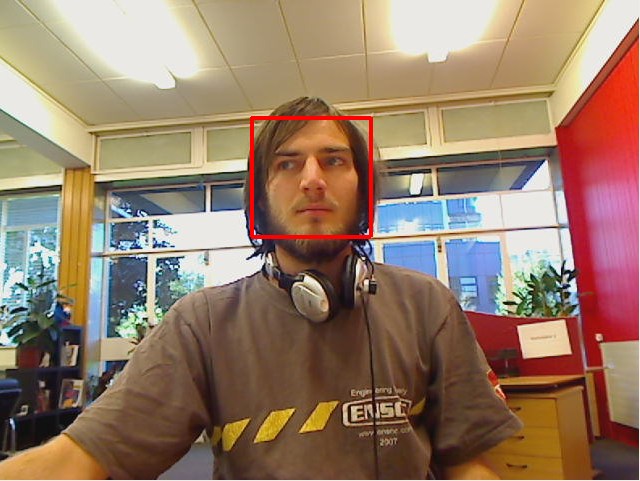
\includegraphics[width=0.45\columnwidth]{report_data/face_detect_one}
\par\end{centering}



}\subfloat[\label{fig:Obscured-opencv-face}Obscured face in frame]{\begin{centering}
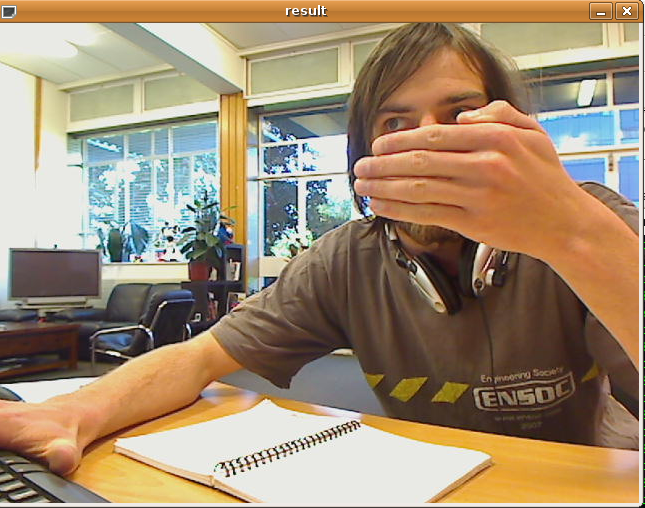
\includegraphics[width=0.45\columnwidth]{report_data/face_detect_obscure}
\par\end{centering}



}

\subfloat[Multiple faces]{\begin{centering}
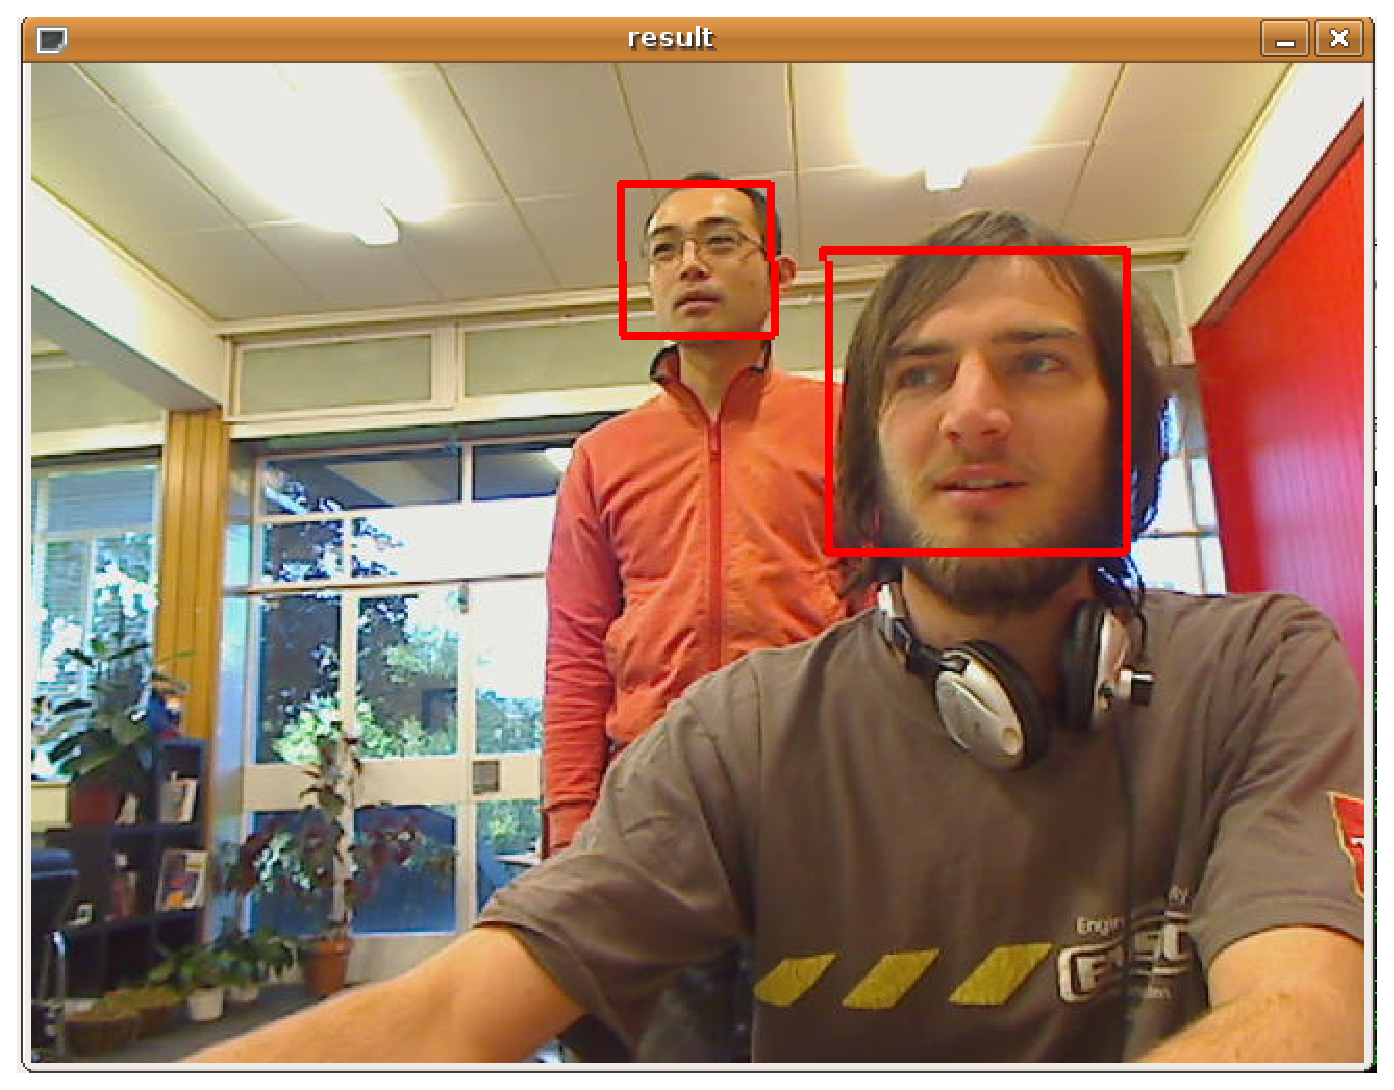
\includegraphics[width=0.45\columnwidth]{report_data/face_detect_two}
\par\end{centering}



}\subfloat[\label{fig:Angled-opencv-face}Rotated face]{\begin{centering}
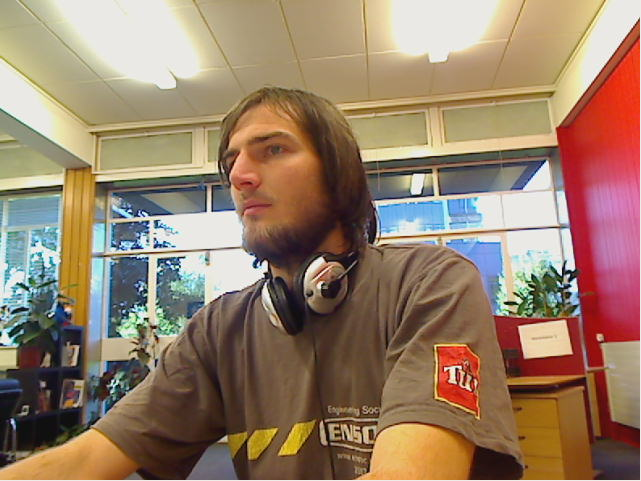
\includegraphics[width=0.45\columnwidth]{report_data/face_detect_sideways}
\par\end{centering}



}

\caption{\label{fig:OpenCV-Face-Detection}OpenCV Face Detection}

\end{figure}


%
\begin{figure}
\begin{centering}
\subfloat[detecting eye and face objects]{\begin{centering}
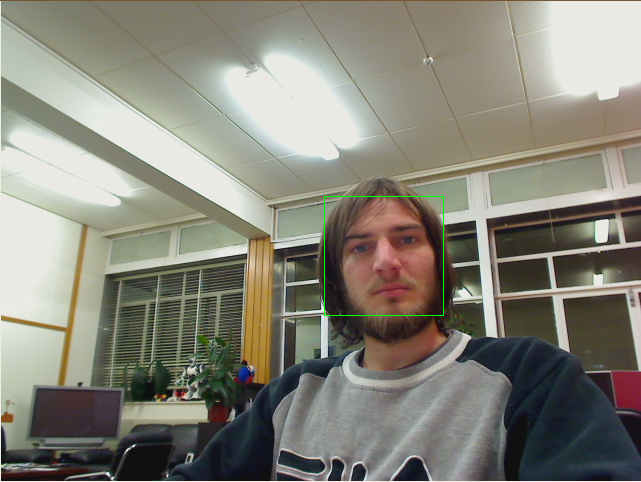
\includegraphics[width=0.4\columnwidth]{report_data/pygame-eye-locate}
\par\end{centering}



}\subfloat[\label{fig:edge-filtering-face}edge filtering and face detection]{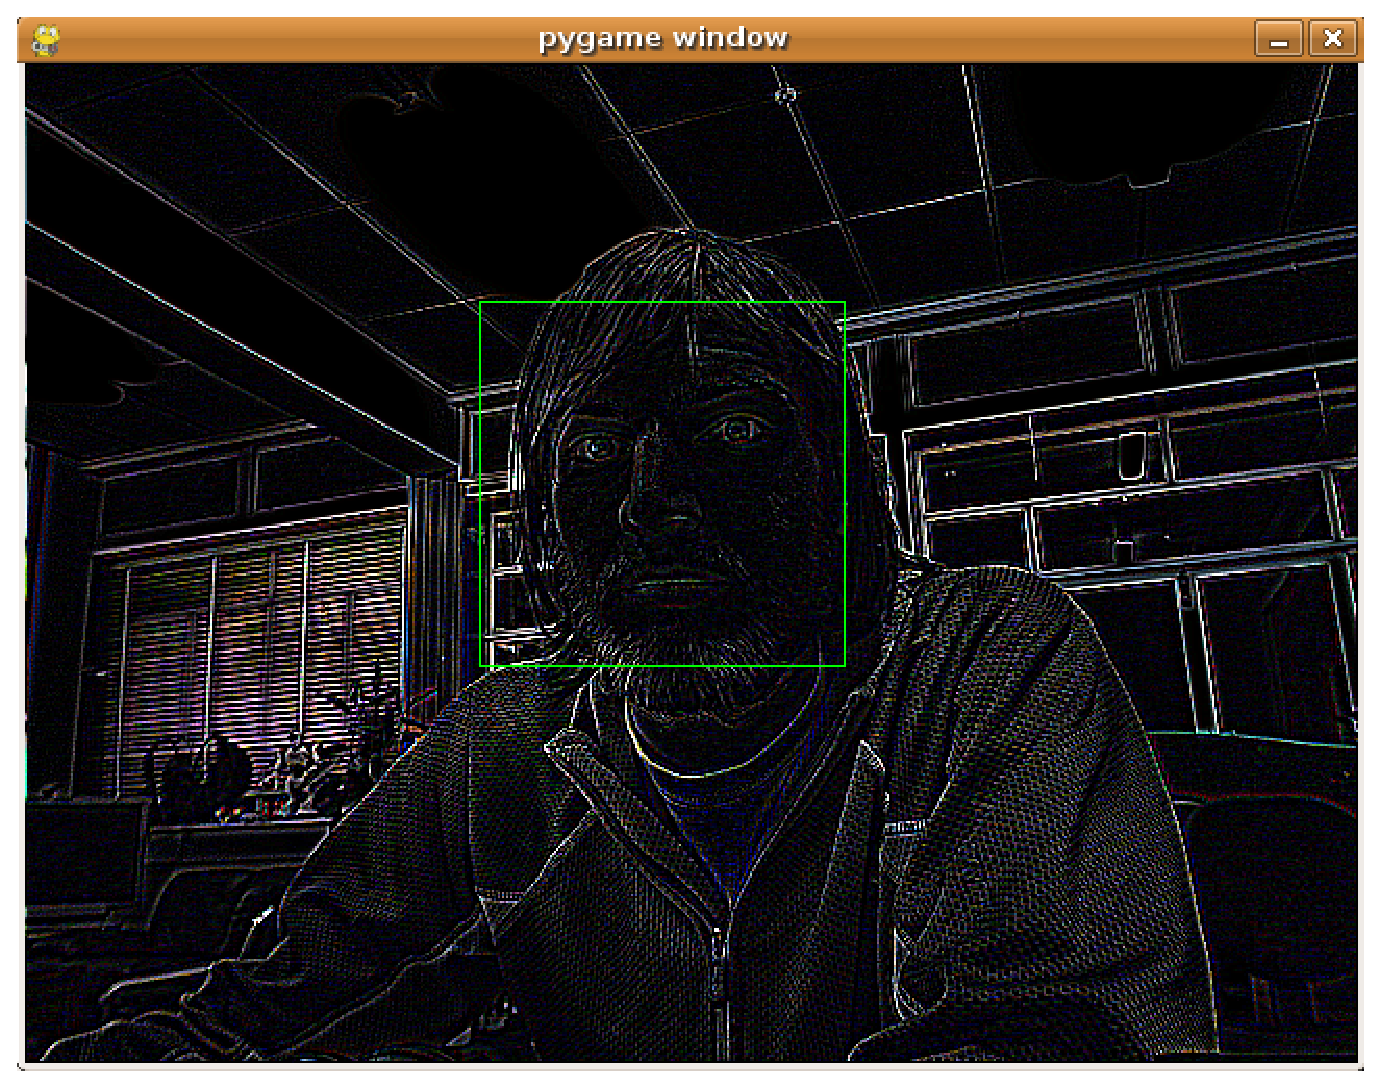
\includegraphics[width=0.4\columnwidth]{report_data/pygame-face-edge}



}
\par\end{centering}

\caption{\label{fig:Pygame-object}Pygame can be used to capture and display
the webcam, while OpenCV does the processing.}



\end{figure}


Figure \ref{fig:Pygame-object} shows an alternative setup; using
the Pygame camera module for image capture, OpenCV for the object
detection and Pygame surfaces for the box rendering and display. Python
really shows its strengths as a glue language here, as the different
libraries are easily used in conjunction with each other. The benifits
from this can be huge, it is very easy for a developer to incorperate
different computer vision tools, even with very limited knowledge
of computer vision.


\section{Related Works}


\begin{itemize}
\item GPUCV\cite{farrugia2006gpucv}\cite{allusse2008gpucv}
\item Pyro - \cite{blank2003pyro} introduced Pyro, a robotics simulation
environment
\item Pygame - a game making package for Python, aimed at new programmers.
It has a camera module and is able to do basic computer vision tasks,
or call on SciPy/NumPy. http://pygame.org
\item Pycam - All code from this project, including framework linking OpenCV
to Pygame and NumPy. http://pycam.googlecode.com
\end{itemize}

\section{Concluding Messages}

Having an interactive interpretter, and using these prototypes in
the final product is a big argument in favor of Python. Most of the
time the reason for slow performance comes down to naive implementations,
which every language is prone to.

A major limitations of using Python would be when the application
is being developed for embedded hardware. 

I would like to thank Rob Ramsey for help with profiling the exectution
of C++ code to ensure acurate timing results were used. Thanks also
to all the developers investing time helping work on the open source
projects OpenCV, Python and SciPy.


\section{Appendix}

%
\begin{algorithm*}
\begin{lyxcode}
\#include~<iostream>~

\#include~\textquotedbl{}videoCapturePlayer.h\textquotedbl{}



CvMat~{*}~gaussianBlur(CvMat~{*}x)\{

//~Filter~with~gaussian~smoothing

~~~~int~filterSize~=~43;

~~~~cvSmooth(x,~x,~CV\_GAUSSIAN,~filterSize);

~~~~return~x;

\}



int~main(~int~argc,~char{*}{*}~argv~)\{

~~~~VideoCapturePlayer~vcp~=~VideoCapturePlayer(\&gaussianBlur);

~~~~vcp.init();~vcp.main();

~~~~return~0;

\}
\end{lyxcode}
\caption{\label{alg:Gaussian-C}Applying Gaussian Blur to web-cam stream from
C++}

\end{algorithm*}


%
\begin{algorithm*}
\begin{lyxcode}
from~VideoCapturePlayer~import~VideoCapturePlayer~as~VCP

from~opencv~import~cv



def~opencvFilt2sigma(size):

~~~~return~((~size{*}0.5~)~-~1){*}0.30~+~0.80



def~gaussianBlur(image):

~~~~\textquotedbl{}\textquotedbl{}\textquotedbl{}Blur~an~image\textquotedbl{}\textquotedbl{}\textquotedbl{}~~~~~

~~~~result~=~cv.cvCreateMat(image.rows,~image.cols,~image.type)

~~~~filterSize~=~43;~sigma~=~opencvFilt2sigma(filterSize)

~~~~cv.cvSmooth(image,~result,~cv.CV\_GAUSSIAN,~filterSize,0,~sigma)

~~~~return~result





VCP(gaussianBlur,~\textquotedbl{}Gaussian~Filtered~Output\textquotedbl{}).main()
\end{lyxcode}
\caption{\label{alg:Gaussian-Python-OpenCV}Gaussian Blurring in Python using
OpenCV}

\end{algorithm*}


%
\begin{algorithm*}
\begin{lyxcode}
from~numpy~import~array,~uint8

from~scipy~import~signal,~ndimage~

from~VideoCapturePlayer~import~VideoCapturePlayer~as~VCP~

from~misc~import~scipyFromOpenCV



def~opencvFilt2sigma(size):

~~~~\textquotedbl{}\textquotedbl{}\textquotedbl{}OpenCV~defaults~to~making~sigma~up~with~this~formula\textquotedbl{}\textquotedbl{}\textquotedbl{}

~~~~return~((~size/2~)~-~1){*}0.30~+~0.80



@scipyFromOpenCV

def~gaussianBlur(np\_image):

~~~~\textquotedbl{}\textquotedbl{}\textquotedbl{}Blur~an~image~with~scipy\textquotedbl{}\textquotedbl{}\textquotedbl{}

~~~~filterSize~=~opencvFilt2sigma(43)

~~~~result~=~ndimage.filters.gaussian\_filter(np\_image,~(filterSize,~filterSize,~1))

~~~~return~result



if~\_\_name\_\_~==~\textquotedbl{}\_\_main\_\_\textquotedbl{}:

~~~~title~=~\textquotedbl{}Gaussian~Filtered~Output\textquotedbl{}

~~~~VCP(gaussianBlur,title=title).main()
\end{lyxcode}
\caption{\label{alg:Gaussian-Python-SciPy}Gaussian Blurring in Python using
SciPy}

\end{algorithm*}


%
\begin{algorithm*}
\begin{lyxcode}
def~gauss\_derivatives(im,~n,~ny=None):

~~~~~\textquotedbl{}\textquotedbl{}\textquotedbl{}~returns~x~and~y~derivatives~of~an~image~using~gaussian

~~~~~~~~~~derivative~filters~of~size~n.~The~optional~argument

~~~~~~~~~~ny~allows~for~a~different~size~in~the~y~direction.\textquotedbl{}\textquotedbl{}\textquotedbl{}

~~~~gx,gy~=~gauss\_derivative\_kernels(n,~sizey=ny)

~~~~imx~=~signal.convolve(im,gx,~mode='same')

~~~~imy~=~signal.convolve(im,gy,~mode='same')

~~~~return~imx,imy



~~~def~compute\_harris\_response(image):

~~~~~~~\textquotedbl{}\textquotedbl{}\textquotedbl{}~compute~the~Harris~corner~detector~response~function

~~~~~~~~for~each~pixel~in~the~image\textquotedbl{}\textquotedbl{}\textquotedbl{}

~~~~~~~~imx,imy~=~gauss\_derivatives(image,~3)

~~~~~~~~gauss~=~gauss\_kern(3)

~~~~~~~~Wxx~=~signal.convolve(imx{*}imx,gauss,~mode='same')

~~~~~~~~Wxy~=~signal.convolve(imx{*}imy,gauss,~mode='same')

~~~~~~~~Wyy~=~signal.convolve(imy{*}imy,gauss,~mode='same')

~~~~~~~~Wdet~=~Wxx{*}Wyy~-~Wxy{*}{*}2

~~~~~~~~Wtr~=~Wxx~+~Wyy

~~~~~~~~return~Wdet~/~Wtr
\end{lyxcode}
\caption{\label{alg:SciPy-Harris-Corner}SciPy Harris Corner Detection}

\end{algorithm*}


%
\begin{algorithm*}
\begin{lyxcode}
def~detectObject(self,img):

~~~~gray~=~cvCreateImage(~cvSize(img.width,img.height),~8,~1~)

~~~~small\_img~=~cvCreateImage(~cvSize(~cvRound~(img.width/self.image\_scale),~

~~~~~~~~~~~~~~~~~~~~~~~~~~~~~~cvRound~(img.height/self.image\_scale)),~8,~1~)

~~~~cvCvtColor(~img,~gray,~CV\_BGR2GRAY~)

~~~~cvResize(~gray,~small\_img,~CV\_INTER\_LINEAR~)

~~~~cvEqualizeHist(~small\_img,~small\_img~)

~~~~cvClearMemStorage(~self.storage~)

~~~~if(~self.cascade~):

~~~~~~~~t~=~cvGetTickCount()

~~~~~~~~objects~=~cvHaarDetectObjects(~small\_img,~self.cascade,~self.storage,

~~~~~~~~~~~~~~~~~~~self.haar\_scale,~self.min\_neighbors,~self.haar\_flags,~self.min\_size~)

~~~~~~~~t~=~cvGetTickCount()~-~t

~~~~~~~~if~verbose:

~~~~~~~~~~~~print~\textquotedbl{}\%i~objects~found,~detection~time~=~\%gms\textquotedbl{}~\%~(objects.total,t/(cvGetTickFrequency(){*}1000.))

~~~~~~~~return~objects
\end{lyxcode}
\caption{\label{alg:OpenCV-Haar-detect}Using the OpenCV Haar Detect Objects
Function}

\end{algorithm*}


%
\begin{algorithm*}
\begin{lyxcode}
\#!/usr/bin/env~python

from~VideoCapturePlayer~import~VideoCapturePlayer~as~VCP

import~numpy

from~scipy.ndimage~import~gaussian\_filter,maximum\_filter

from~numpy~import~array,ones,zeros,nonzero

from~opencv~import~cv



def~harrisResponse(image,~n~=~15):

~~\textquotedbl{}\textquotedbl{}\textquotedbl{}Modified~from~PyVision~example

~~\textquotedbl{}\textquotedbl{}\textquotedbl{}

~~gray~=~cv.cvCreateImage(~cv.cvGetSize(image),~8,~1~)

~~corners~=~cv.cvCreateImage(~cv.cvGetSize(image),~32,~1~)

~~cv.cvCvtColor(~image,~gray,~cv.CV\_BGR2GRAY~)

~~cv.cvCornerHarris(gray,corners,~n)

~~

~~\#~Filter~the~response~and~draw~points

~~buffer~=~corners.imageData

~~corners~=~numpy.frombuffer(buffer,numpy.float32)

~~corners~=~corners.reshape(corners.height,corners.width)

~~corners~=~corners.transpose()

~~

~~footprint~=~ones((n,n))

~~mx~=~maximum\_filter(corners,~footprint~=~footprint)

~~local\_maxima~=~(corners~==~mx)~{*}~(corners~!=~zeros(corners.shape))

~~points~=~nonzero(local\_maxima)

~~del~local\_maxima

~~points~=~array({[}points{[}0{]},points{[}1{]}{]}).transpose()

~~L~=~{[}{]}

~~for~each~in~points:

~~~~L.append((corners{[}each{[}0{]},each{[}1{]}{]},each{[}0{]},each{[}1{]},None))

~~~~i~=~cv.cvPoint(int(each{[}0{]}),int(each{[}1{]}))

~~~~cv.cvCircle(image,~i,~2,~cv.CV\_RGB(0,0,200),3~)



~~return~image



title~=~\textquotedbl{}Harris~Feature~Detection\textquotedbl{}

VCP(harrisResponse,~title).main()
\end{lyxcode}
\caption{\label{alg:Harris-Detection-opencv}Harris Detection in OpenCV}

\end{algorithm*}


%
\begin{algorithm*}
\begin{lyxcode}


~~~~differenceImage~~=~cv.cvCloneMat(~image~)

~~~~cv.cvAbsDiff(~image,~original,~differenceImage~)

~~~~

~~~~cv.cvThreshold(~differenceImage,~differenceImage,~32,~255,~cv.CV\_THRESH\_BINARY~)

~~~~cv.cvSmooth(differenceImage,~differenceImage,~cv.CV\_MEDIAN,~15)



~~~~temp~~=~cv.cvCloneMat(~image)

~~~~cv.cvSetZero(temp)

~~~~

~~~~for~row\_n~in~xrange(image.rows):

~~~~~~~~for~col\_n~in~xrange(image.cols):

~~~~~~~~~~~~if~differenceImage{[}row\_n,col\_n{]}{[}0{]}~>~0~\textbackslash{}

~~~~~~~~~~~~or~differenceImage{[}row\_n,col\_n{]}{[}1{]}~>~0~\textbackslash{}

~~~~~~~~~~~~or~differenceImage{[}row\_n,col\_n{]}{[}2{]}~>~0:

~~~~~~~~~~~~~~~~temp{[}row\_n,col\_n{]}~=~image{[}row\_n,col\_n{]}

~~~~

~~~~return~temp


\end{lyxcode}
\caption{\label{alg:back-Python-imple}Python implementaition of background
subtraction}

\end{algorithm*}


%
\begin{algorithm*}
/{*} g++ -O3 -Wall

`pkg-config --cflags opencv` 

`pkg-config --libs opencv` -o bg\_sub 

bg\_sub.cxx videoCapturePlayer.cxx

{*}/

\#include <iostream>

\#include \textquotedbl{}videoCapturePlayer.h\textquotedbl{}

CvMat {*}original;

CvMat {*} bg\_subtract(CvMat {*}x)

\{

static int n = 0;

++n;

if( n == 3) original = cvCloneMat( x );

if( n < 4) return x;

if(n\%100 == 0) std::cout <\textcompwordmark{}< \textquotedbl{}100
frames\textquotedbl{} <\textcompwordmark{}< std::endl;

CvMat {*} differenceImage = cvCloneMat( x );

cvAbsDiff( x, original, differenceImage );

//CV\_THRESH\_TOZERO

CvMat {*} temp = cvCloneMat( x );

cvSetZero(temp);

cvThreshold( differenceImage, temp, 32, 255, CV\_THRESH\_BINARY );

// median filter out the salt \& pepper noise in the difference image

cvSmooth(temp, temp, CV\_MEDIAN, 5);

cvSetZero(differenceImage);

cvAnd(x, temp, differenceImage ); // NOTE DIFF FROM PYTHON

return differenceImage;

\}

VideoCapturePlayer vcp = VideoCapturePlayer(\&bg\_subtract);

vcp.init(); vcp.main();



\caption{C++ Background Subtraction}



\end{algorithm*}


%
\begin{algorithm*}
\begin{lyxcode}
\#!/usr/bin/env~python

from~\_\_future\_\_~import~division

from~opencv~import~cv,~highgui~as~hg

import~time

import~logging

verbosity~=~logging.INFO

profiling~=~False

logging.basicConfig(filename=None,level=verbosity,)

class~VideoCapturePlayer(object):

~~~~\textquotedbl{}\textquotedbl{}\textquotedbl{}

~~~~A~VideoCapturePlayer~object~is~an~encapsulation~of~

~~~~the~display~of~a~video~stream.~

~~~~

~~~~A~process~can~be~given~(as~a~function)~that~is~run

~~~~on~every~frame~between~capture~and~display.

~~~~

~~~~For~example~a~filter~function~that~takes~and~returns~a~

~~~~cvMat~can~be~given.~This~player~will~take~the~webcam~image,~

~~~~pass~it~through~the~filter~then~display~the~result.

~~~~

~~~~>\textcompwordmark{}>\textcompwordmark{}>~vcp~=~VideoCapturePlayer()~~\#~Open~the~webcam.

~~~~>\textcompwordmark{}>\textcompwordmark{}>~vcp.main()~~\#~should~start~capturing~and~showing~the~webcam

~~~~

~~~~And~defining~and~giving~a~process~function~to~the~player:

~~~~

~~~~>\textcompwordmark{}>\textcompwordmark{}>~def~drawBox(x):

~~~~....~~~~pt1,~pt2~=~cv.CvPoint(),~cv.CvPoint()

~~~~....~~~~pt1.x~=~pt1.y~=~200

~~~~....~~~~pt2.x~=~pt2.y~=~250

~~~~....~~~~cv.cvRectangle(~x,~pt1,~pt2,~cv.CV\_RGB(30,0,200)~)

~~~~....~~~~return~x

~~~~>\textcompwordmark{}>\textcompwordmark{}>~vcp~=~VideoCapturePlayer(processFunction=drawBox)

~~~~>\textcompwordmark{}>\textcompwordmark{}>~vcp.main()

~~~~

~~~~\textquotedbl{}\textquotedbl{}\textquotedbl{}

~~~

~~~~def~\_\_init\_\_(self,~processFunction~=~None,~title~=~\textquotedbl{}Video~Capture~Player\textquotedbl{},~show=True)

~~~~~~~~t\_begin~=~time.time()

~~~~~~~~self.processFunction~=~processFunction

~~~~~~~~self.title~=~title

~~~~~~~~self.show~=~show

~~~~~~~~if~self.show~is~True:

~~~~~~~~~~~~self.display~=~hg.cvNamedWindow(self.title)

~~~~~~~~try:

~~~~~~~~~~~~self.camera~=~hg.cvCreateCameraCapture(0)

~~~~~~~~except:

~~~~~~~~~~~~print(\textquotedbl{}Couldn't~open~camera~device,~is~it~connected?\textquotedbl{})

~~~~~~~~~~~~hg.cvDestroyWindow(title)

~~~~~~~~~~~~raise~SystemExit

~~~~~~~~

~~~~~~~~\#~Take~a~frame~to~get~props~and~use~in~testing

~~~~~~~~self.snapshot~=~cv.cvCloneMat(~hg.cvQueryFrame(~self.camera~)~)

~~~~~~~~\#~check~that~we~got~an~image,~otherwise~try~again.

~~~~~~~~for~i~in~xrange(100):

~~~~~~~~~~~~if~self.snapshot~is~not~None:~break

~~~~~~~~~~~~self.snapshot~=~hg.cvQueryFrame(~self.camera~)

~~~~~~~~

~~~~def~process(self,~take\_new\_image=True):

~~~~~~~~\textquotedbl{}\textquotedbl{}\textquotedbl{}We~will~take~a~snapshot,~optionally~do~some~arbitrary~process~(eg~in~numpy/scipy)

~~~~~~~~then~display~it.

~~~~~~~~\textquotedbl{}\textquotedbl{}\textquotedbl{}

~~~~~~~~try:

~~~~~~~~~~~~if~take\_new\_image:

~~~~~~~~~~~~~~~~logging.debug(\textquotedbl{}capturing~an~image\textquotedbl{})

~~~~~~~~~~~~~~~~self.snapshot~=~cv.cvCloneMat(~hg.cvQueryFrame(~self.camera)~)

~~~~~~~

~~~~~~~~~~~~if~self.processFunction~is~not~None:

~~~~~~~~~~~~~~~~logging.debug(\textquotedbl{}Sending~image~to~process~function\textquotedbl{})

~~~~~~~~~~~~~~~~res~=~self.processFunction(self.snapshot)

~~~~~~~~~~~~~~~~logging.debug(\textquotedbl{}Received~result~from~processing~function\textquotedbl{})

~~~~~~~~~~~~~~~~assert~isinstance(res,cv.CvMat),~\textquotedbl{}Not~CvMat\textquotedbl{}

~~~~~~~~~~~~~~~~self.snapshot~=~res

~~~~~~~~~~~~~~~~~~~~~~~

~~~~~~~~~~~~if~self.show:

~~~~~~~~~~~~~~~~hg.cvShowImage(~self.title,~self.snapshot~)

~~~~~~~~except~Exception,~e:

~~~~~~~~~~~~\#~If~something~goes~wrong~make~sure~we~close~the~window

~~~~~~~~~~~~logging.error(\textquotedbl{}Error~in~processing~image:~\%s\textquotedbl{}~\%~e)

~~~~~~~~~~~~hg.cvDestroyWindow(self.title)

~~~~~~~~~~~~raise~SystemExit



~~~~def~main(self):

~~~~~~~~\textquotedbl{}\textquotedbl{}\textquotedbl{}

~~~~~~~~Run~and~time~the~main~loop.

~~~~~~~~\textquotedbl{}\textquotedbl{}\textquotedbl{}

~~~~~~~~logging.info(\textquotedbl{}Starting~main~video~capture~loop~now,~press~'q'~to~quit\textquotedbl{})

~~~~~~~~key~=~hg.cvWaitKey(1)

~~~~~~~~

~~~~~~~~num\_frames~=~0

~~~~~~~~start\_time~=~time.time()

~~~~~~~~

~~~~~~~~while(key~is~not~\textquotedbl{}q\textquotedbl{}~and~key~!=~'\textbackslash{}x1b'):

~~~~~~~~~~~~num\_frames~+=1

~~~~~~~~~~~~self.process()

~~~~~~~~~~~~key~=~hg.cvWaitKey(5)

~~~~~~~~~~~~

~~~~~~~~total\_time~=~float(time.time())~-~float(start\_time)

~~~~~~~~

~~~~~~~~logging.debug(\textquotedbl{}Main~loop~complete\textquotedbl{})

~~~~~~~~logging.debug(\textquotedbl{}Total~time~took~\%e\textquotedbl{}~\%~total\_time)

~~~~~~~~

~~~~~~~~logging.info(\textquotedbl{}Average~time~per~frame:~\%e\textquotedbl{}~\%~(total\_time/num\_frames)~)

~~~~~~~~logging.info(\textquotedbl{}Average~frames~per~second:~\%f\textquotedbl{}~\%~(num\_frames/total\_time)~)



def~drawBox(x):

~~~~\textquotedbl{}\textquotedbl{}\textquotedbl{}

~~~~This~is~a~template~for~a~function~that~can~be~fed~into~VideoCapturePlayer

~~~~It~must~take~a~CvMat,~and~return~a~CvMat.

~~~~It~draws~a~rectangle~on~the~screen.\textquotedbl{}\textquotedbl{}\textquotedbl{}

~~~~pt1,~pt2~=~cv.CvPoint(),~cv.CvPoint()

~~~~pt1.x~=~pt1.y~=~200

~~~~pt2.x~=~pt2.y~=~250

~~~~cv.cvRectangle(~x,~pt1,~pt2,~cv.CV\_RGB(30,0,200)~)

~~~~return~x



if~\_\_name\_\_~==~\textquotedbl{}\_\_main\_\_\textquotedbl{}:

~~~~logging.info(\textquotedbl{}Starting~the~example~VideoCapturePlayer\textquotedbl{})

~~~~\#vcp~=~VideoCapturePlayer(processFunction=drawBox)

~~~~vcp~=~VideoCapturePlayer()

~~~~vcp.main()




\end{lyxcode}
\caption{Python implementaiton of the VideoCaptureClass}



\end{algorithm*}


\bibliographystyle{ieeetr}
\bibliography{report_data/database}

\end{document}
